\section{\framework{} Methodology}
\label{sec:methodology}

We now provide the methodology to achieve the goal of deceiving user data fed to the apps without rooting the device or altering the source of the apps.

\subsection{Background on Hooking}
In Android, users cannot typically modify app or OS behavior, but \textit{hooking} provides a practical method to alter execution flow by injecting new instructions.

Hooking can be either static or dynamic. Static hooking modifies an app's bytecode or injects shared libraries before execution, creating permanent changes that can be detected via digital signature verification. Dynamic hooking, on the other hand, applies “hooks” at runtime by altering volatile memory, allowing temporary modifications based on the execution context. Android's Dalvik VM utilizes Dynamic Linkers' "virtual method table" to locate method calls, enabling \textit{Call Diversion} to inject hooks into the method lookup table.

\begin{figure}[t]
    \centering
    \begin{subfigure}{0.48\linewidth}
        \vspace{7mm}
        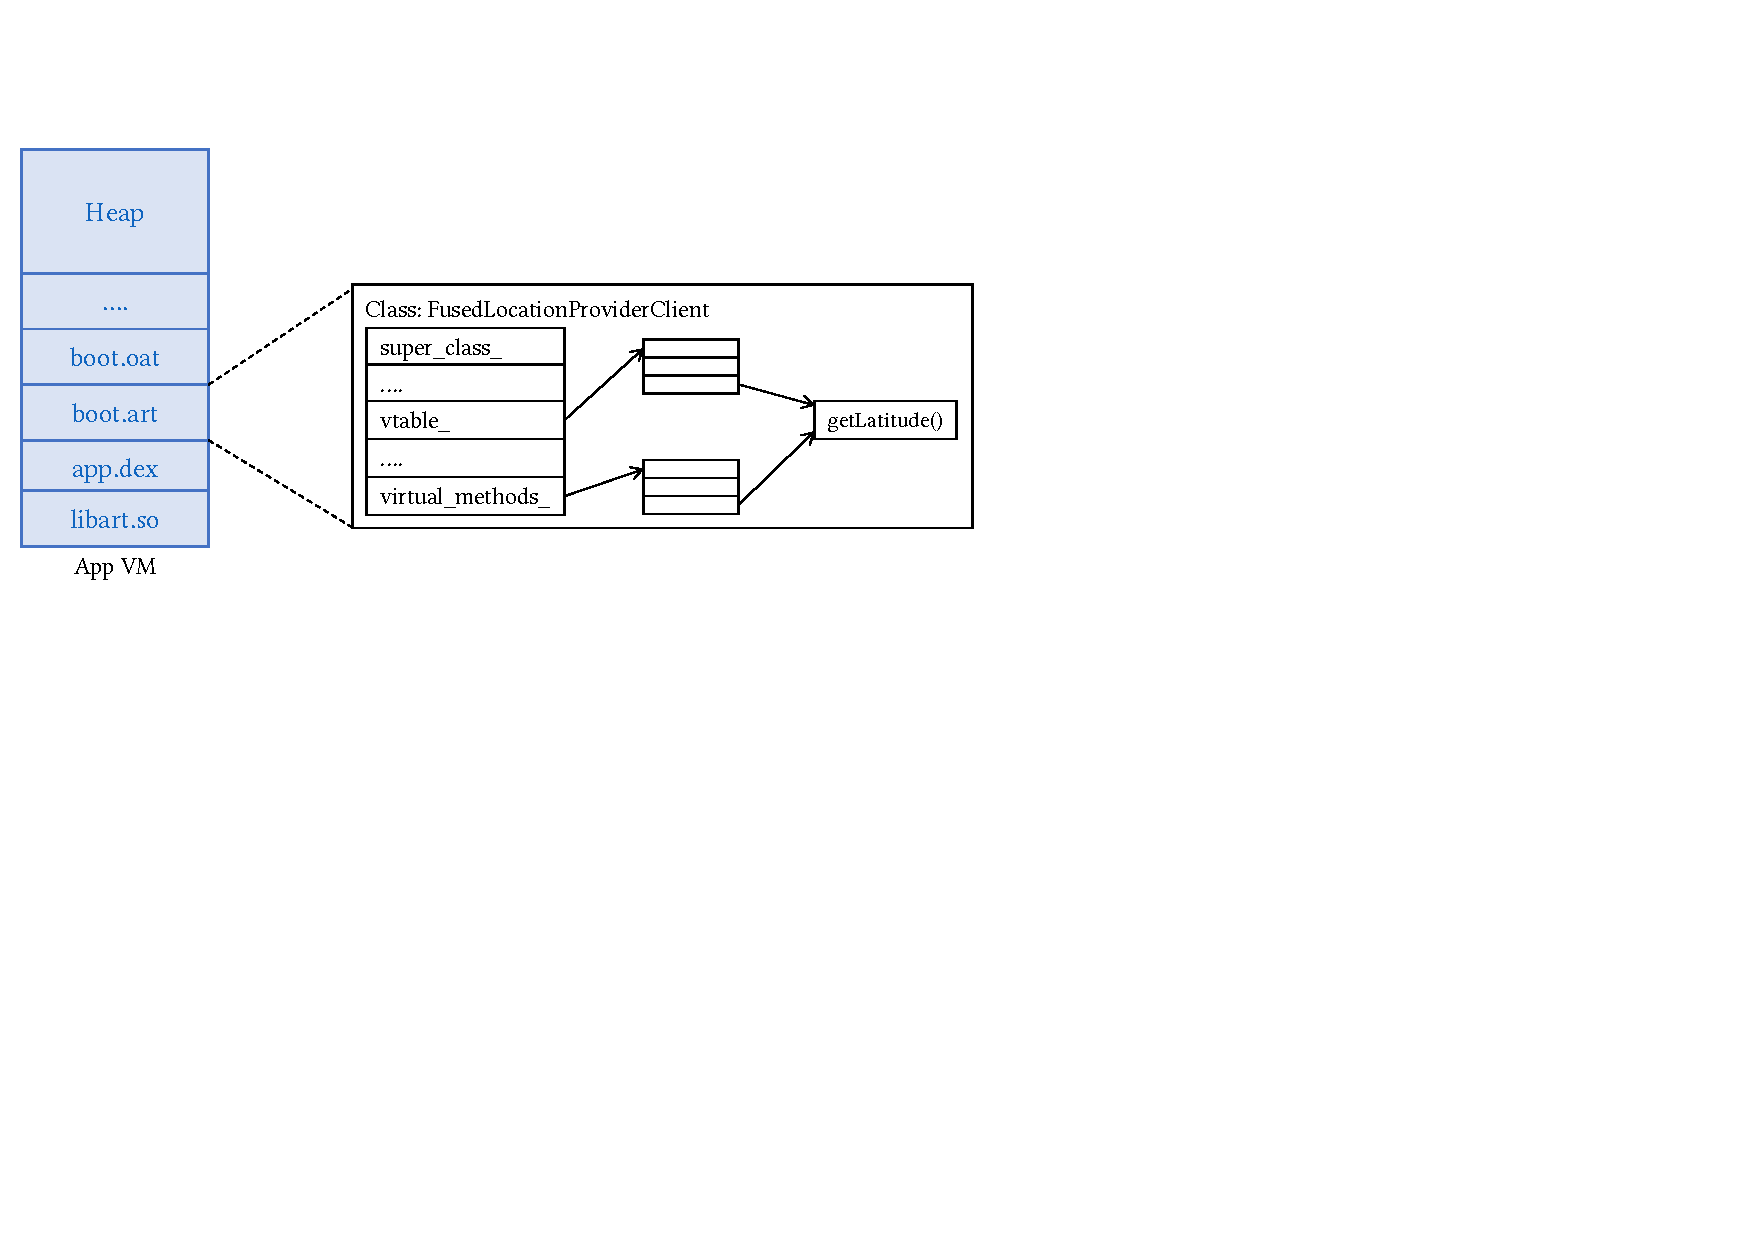
\includegraphics[width=\linewidth]{Figures/Background/virtual_memory_without_deceiver.pdf}
        \caption{Original method call.}
        \label{fig:vrtulMemMthdCall_woFr}
    \end{subfigure}
    \begin{subfigure}{0.48\linewidth}
        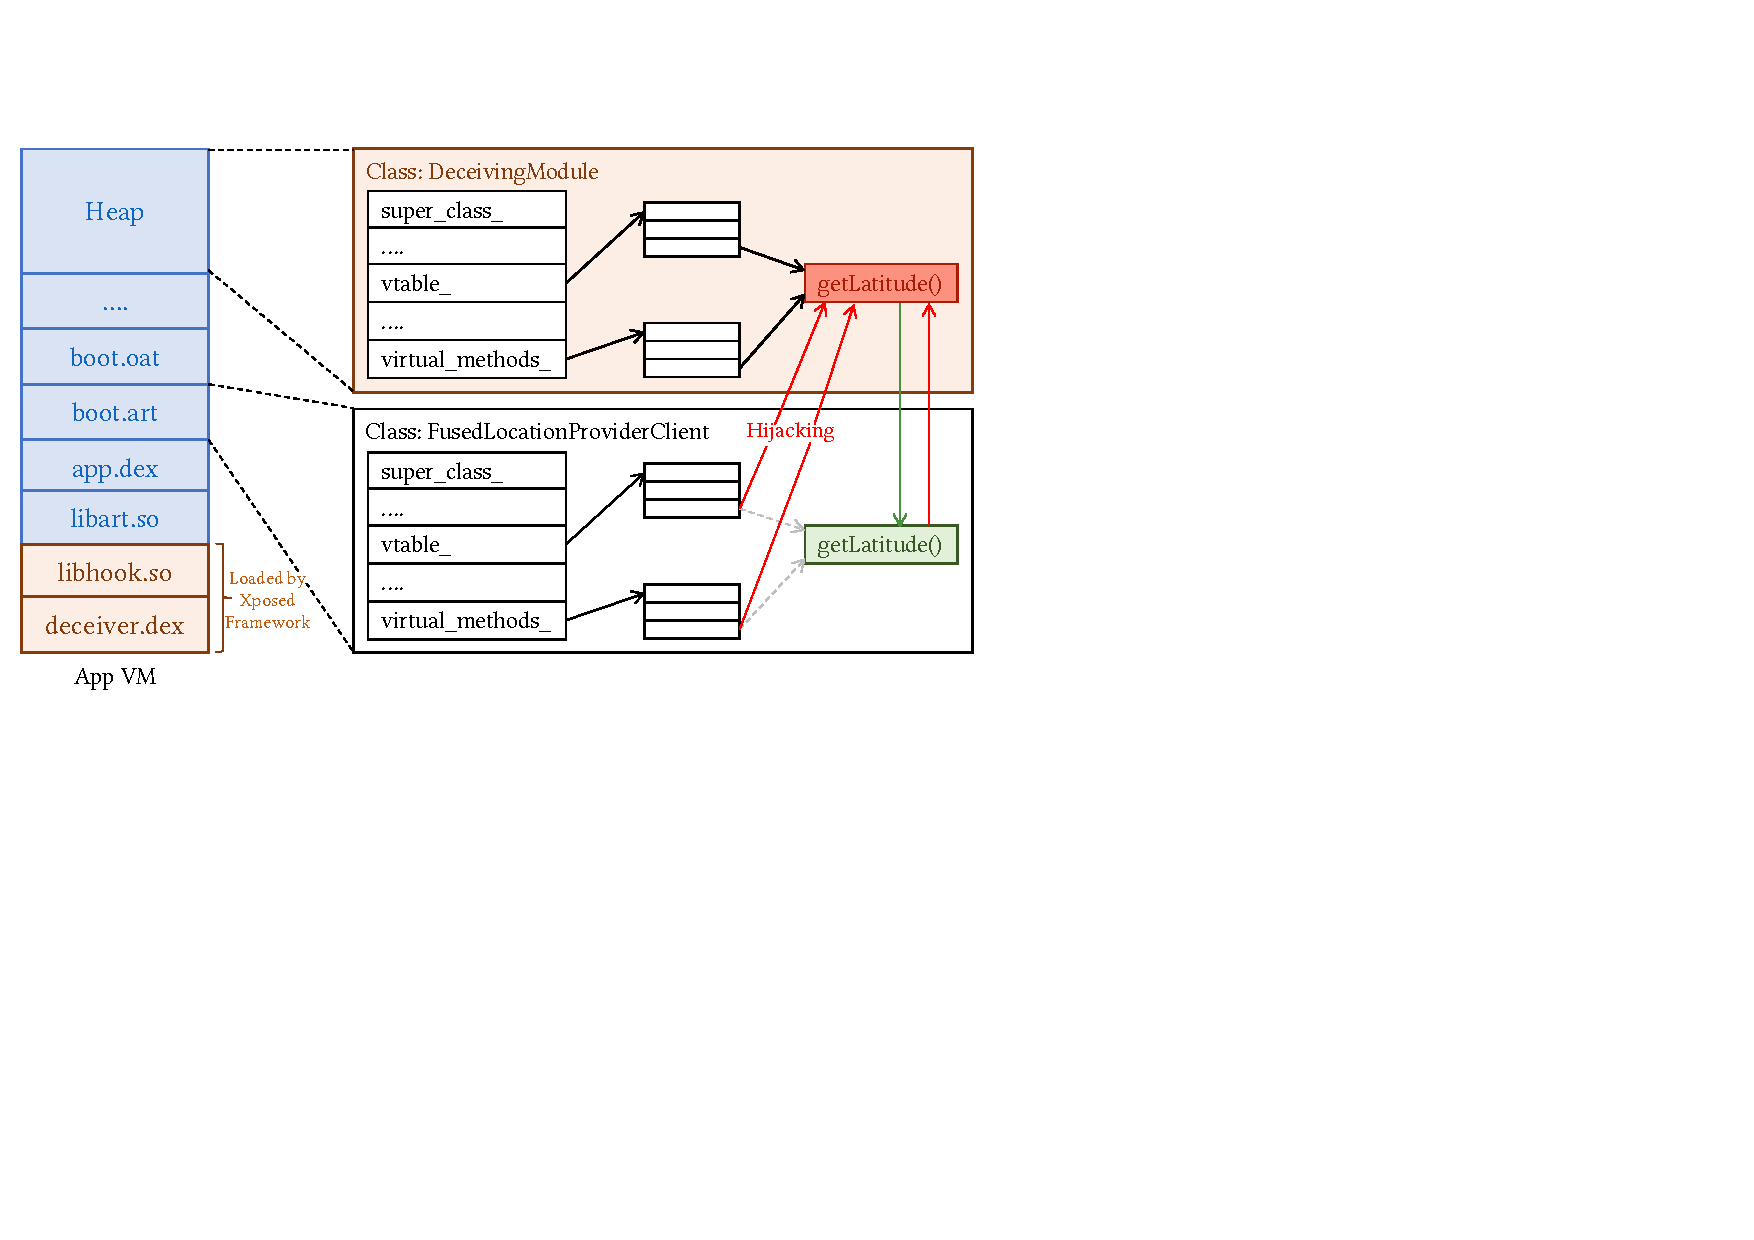
\includegraphics[width=\linewidth]{Figures/Background/virtual_memory_with_deceiver.pdf}
        \caption{Method call with \framework{}.}
        \label{fig:vrtulMemMthdCall_wFr}
    \end{subfigure}
    \caption{Example illustrating how the Xposed module class method hijacks the original method call.}
    \label{fig:vrtulMemMthdCall}
\end{figure}

Figure \ref{fig:vrtulMemMthdCall} illustrates dynamic hooking in Android using \texttt{getLatitude} method of \texttt{Location} class. In Figure \ref{fig:vrtulMemMthdCall_woFr}, the standard method call process is shown, where the target app's virtual memory consists of heap space and files loaded by the \textit{Zygote} process. Zygote, initialized during OS boot, serves as a template with preloaded Java shared libraries, facilitating app launches.

The \texttt{boot.oat} and \texttt{boot.art} files optimize boot speed by storing frequently used class source code and a pre-initialized heap. The target class's heap resides in \texttt{boot.art}, while \texttt{app.dex} and \texttt{libart.so} store the app's Dalvik Executable code and shared libraries. When the app calls a target method, the system retrieves the method's address from virtual tables in the heap and executes it.

Figure \ref{fig:vrtulMemMthdCall_wFr} illustrates the hooking process, where the hooking module loads \texttt{libhook.so} into the app's memory. It then injects hooks from \texttt{hook.dex} as Dalvik Executables. \texttt{libhook.so} modifies the heap by replacing virtual table entries of target classes with hooking method addresses. Consequently, method calls are redirected to the hooking methods, which then invoke the original method at the end.

% \begin{lstlisting}[caption={Kotlin code to deceive Clipboard permission data with the data defined by user in \textit{Deceit} policies.},label={lst:clipboardDeceiver},language=Kotlin,float=*]
class SpoofingModule: IXposedHookLoadPackage {
    companion object {
        fun getClass(clsName: String): Class<*> = Class.forName(clsName, false, lpparam.classLoader)    
    }
    
    @Throws(Throwable::class)
    override fun handleLoadPackage(lpparam: XC_LoadPackage.LoadPackageParam) {
        hookAllMethods(getClass(ClipData.CREATOR.javaClass.name), "createFromParcel", XC_MethodHook() {
            @Throws(Throwable::class)
            override fun beforeHookedMethod(param: MethodHookParam) {
                val uri = Uri.parse("content://com.xposedModule.provider/deceitSettings")
                val cursor = context.contentResolver.query(uri, null, null, null, null) ?: return
                val blockClipboard = cursor.getInt(cursor.getColumnIndex("blockClipboard")
                cursor.close()
                if(blockClipboard) param.result = null
            }

            @Throws(Throwable::class)
            override fun afterHookedMethod(param: MethodHookParam) {
                param.result ?: return
                val uri = Uri.parse("content://com.xposedModule.provider/deceits")
                val cursor = context.contentResolver.query(uri, null, null, null, null) ?: return
                val clipboardLabel = cursor.getString(getColumnIndex("clipboardLabel")) ?: "dummyLabel"
                val clipboardText = cursor.getString(getColumnIndex("clipboardText")) ?: "dummyText"  
                cursor.close()
                param.result = ClipData.newPlainText(clipboardLabel, clipboardText)
            }       
        })   
    }
}
\end{lstlisting}

\subsection{Hooking on Non-Rooted Device}

App hooking is the most effective method for spoofing user data, but non-rooted devices lack access to root or system process hooking. To enable hooking, root access to the \textit{Zygote} process is required.

We achieve this using \textit{adb} (Android Debug Bridge), which provides privileged system API access but only while the device is connected. To bypass this limitation, we leverage Shizuku, which runs a dedicated process with shell-level permissions, acting as a proxy between apps and the OS—sufficient for hooking target apps. With Shizuku, we use LSPatch, an Xposed framework for non-rooted devices, to inject hooks into app processes. This allows users to define custom behavior within the Xposed module, ensuring target apps function as desired. Both Shizuku and LSPatch are open-source and user-controlled, granting root privileges only to selected modules and apps, preserving security.

\subsection{Spoofing User Data with Hooking}

Listing \ref{lst:clipboardDeceiver} illustrates how clipboard data can be spoofed using hooking. Apps typically retrieve clipboard content via \texttt{ClipboardManager.getPrimaryClip()}, but modifying its output requires hooking multiple methods. A more efficient alternative is hooking \texttt{ClipData.CREATOR.createFromParcel()}, as it is the final method invoked to return clipboard data. This is achieved using Xposed's \texttt{handleLoadPackage()} (Line~7).

With this approach, clipboard data can be blocked or modified before reaching target apps. The before hook (Lines 11-15) blocks clipboard access by retrieving the user's preference via \textit{ContentProvider} (Lines 11-13). If blocking is enabled (Line 15), the function returns a null object, preventing the original method from executing.

Similarly, the after hook (Lines 20-26) replaces clipboard content with user-defined spoofed data. The spoofed text is retrieved from \textit{ContentProvider} (Lines 21-24) and used to initialize a new \texttt{ClipData} object (Line 26).

\framework{} also offers various permission-spoofing policies. For example, it blurs images when an app accesses the camera in the background, detected via \texttt{ActivityManager}, by manipulating pixel data. Another policy injects noise into the audio feed if an app requests microphone access without a valid reason.

\subsection{\framework{} and its Robustness}
This section outlines \framework{}'s approach to spoofing user data and evaluates its effectiveness in real-world applications, demonstrating its robustness.

\mysubsubsection{Robust Mechanism} \framework{} employs dynamic hooking to modify user data in volatile memory without altering disk storage, making it undetectable via APK signatures or Google's Play Integrity API. Instead of revoking permissions, it contextually spoofs data, ensuring app stability and a crash-proof user experience.

\mysubsubsection{Real-World Evaluation} \framework{} was tested on 50 Google Play Store apps and 20 pre-installed Android apps. All permissions were granted, and each app was manually used for 20 minutes on a \textit{Samsung Galaxy M21} (2.3 GHz octa-core processor, 4 GB RAM, Android 12). Results were verified through visual confirmation of spoofed data and \framework{}'s logs.

\begin{figure}[t]
    \centering
    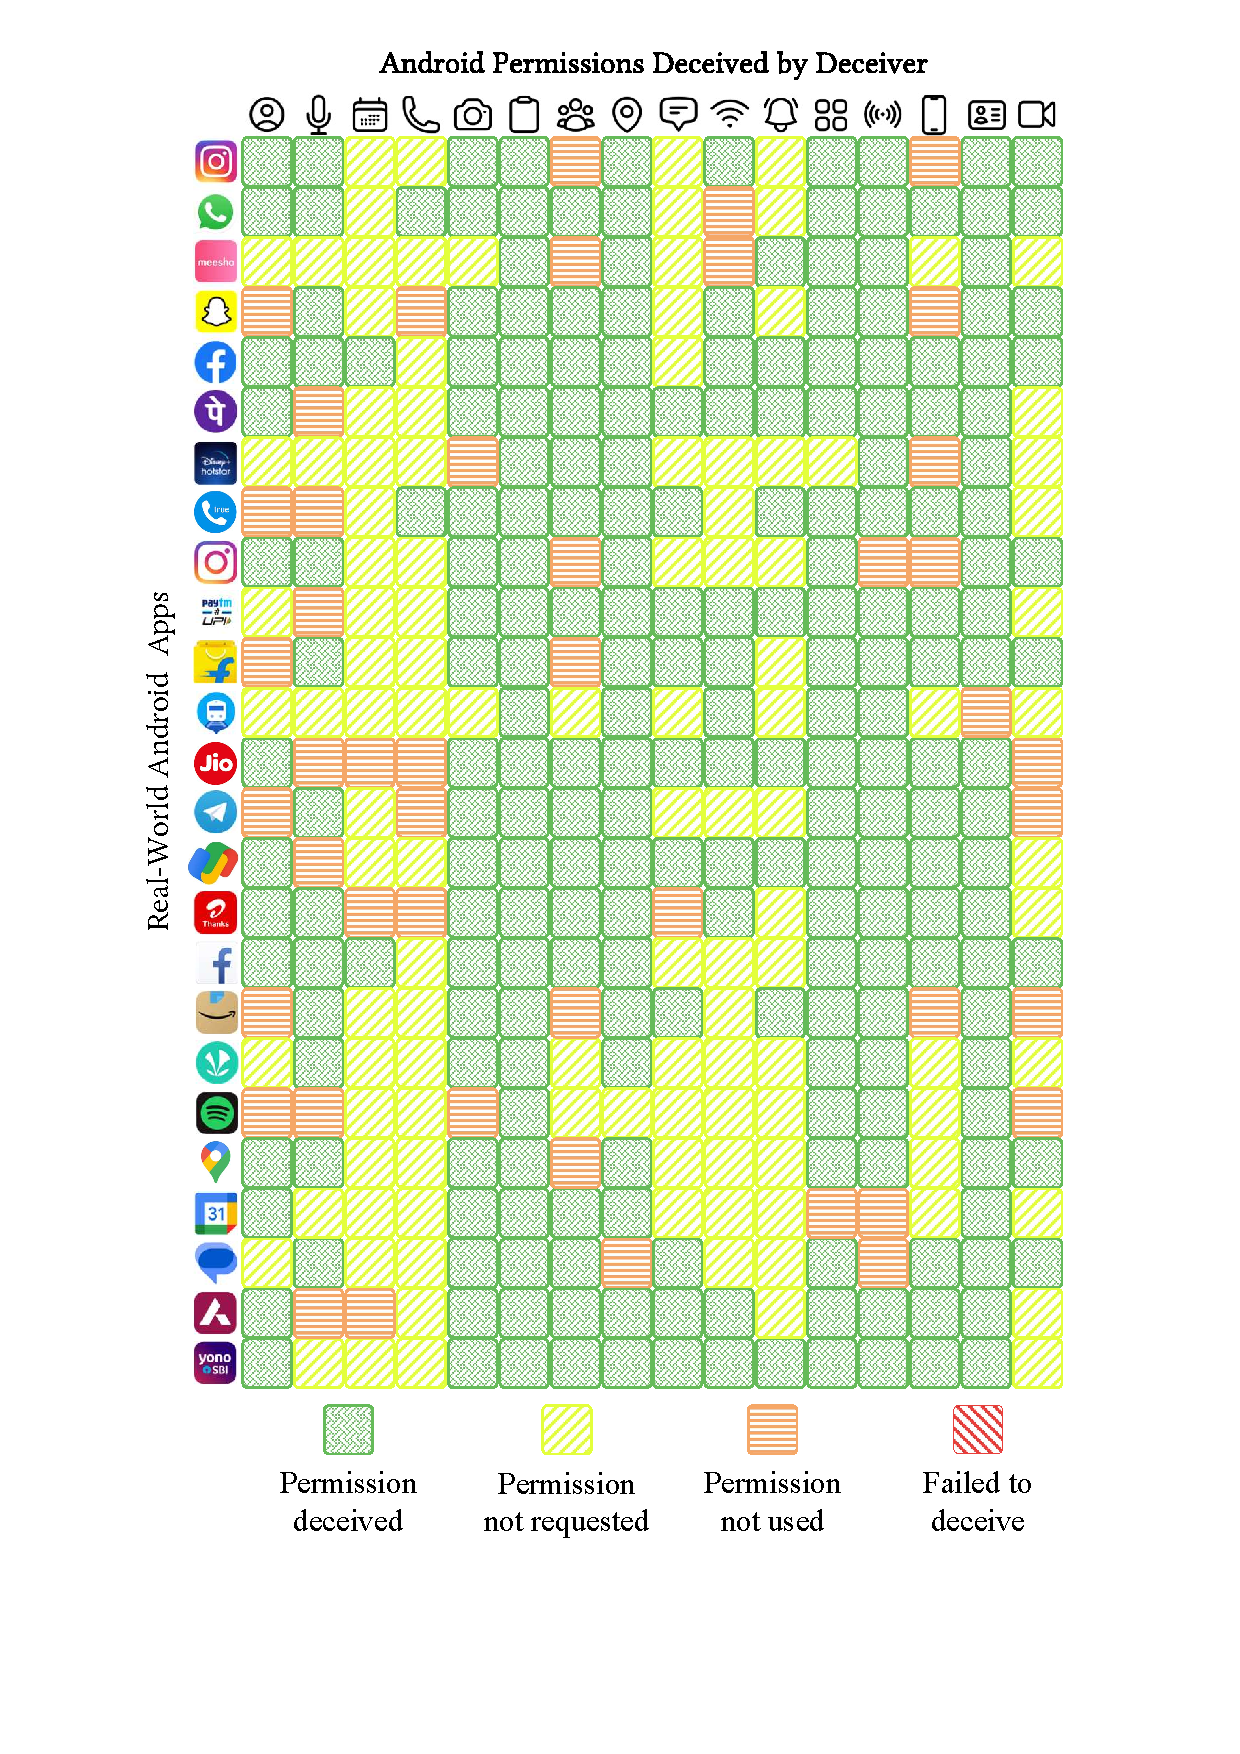
\includegraphics[width=0.6\linewidth]{Figures/Introduction/heatmap.pdf}
    \caption{Heatmap illustrating status of user data deceived for various popular apps by \framework{}.}
    \label{fig:intro_heatmap}
\end{figure}

Figure \ref{fig:intro_heatmap} presents \framework{}'s performance, where dark green areas indicate successfully deceived permissions, while light green, orange, and red represent permissions that were not requested, not used, or not deceivable, respectively. Out of 678 requested permissions, \framework{} successfully spoofed 78.32\%, while 21.68\% could not be verified as they were not explicitly utilized. The results confirm \framework{}'s robustness, as no app crashed, and all functioned as expected.

\mysubsubsection{Hooking Hidden APIs} Certain permissions, like those involving sensors, rely on \textit{Android Non-SDK Interfaces} (\textit{Hidden APIs}) such as \texttt{InputSensorInfo}, which are restricted for \textit{JNI} and \textit{Java Reflections}. \framework{} circumvents these restrictions using \textit{LSPlant} to instantiate classes with spoofed data. Notably, 23.16\% of successful spoofing was achieved through Hidden API hooking, demonstrating \framework{}'s ability to bypass Android's access limitations.

\mysubsubsection{Secure and Isolated Operation} \framework{} requires only the \textit{Query All Packages} permission, a non-runtime (normal) permission, to enhance its privacy protection features. It operates entirely offline, ensuring no external connections and maintaining a secure, trustworthy environment.
